\section{1174027 - Harun Ar - Rasyid}
\subsection{Introducing Python}
\hfill\break
Python adalah bahasa pemrograman yang kuat, dinamis, dan digunakan dalam berbagai macam aplikasi. \\
Beberapa fitur-fiturnya adalah sebagai berikut:
\begin{itemize}
    \item Sintaks yang mudah dibaca dan jelas.
    \item Perpustakaan standar yang sangat luas.
    \item Pengembangan Cepat dan debugging yang mudah dipelajari.
\end{itemize}
\subsection{Help Function}
\hfill\break
Python interpreter sudah menyediakan sistem bantuan yang valid.
\begin{enumerate}
    \item Help(object)
    \lstinputlisting[firstline=7, lastline=8]{src/kelompok3/1/1.py}
    \begin{figure}[H]
        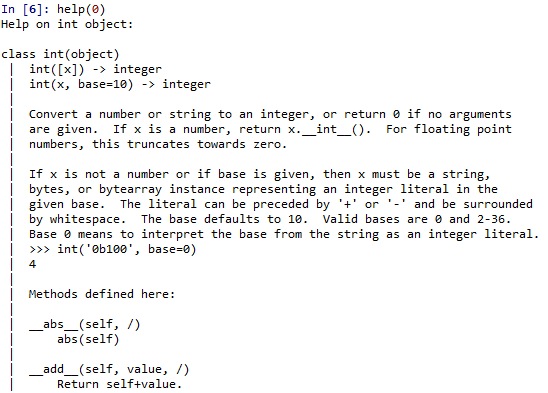
\includegraphics[width=4cm]{figures/kelompok3/1/1.png}
        \centering
        \caption{Hasil Dari Help bagian 1}
    \end{figure}
    \begin{figure}[H]
        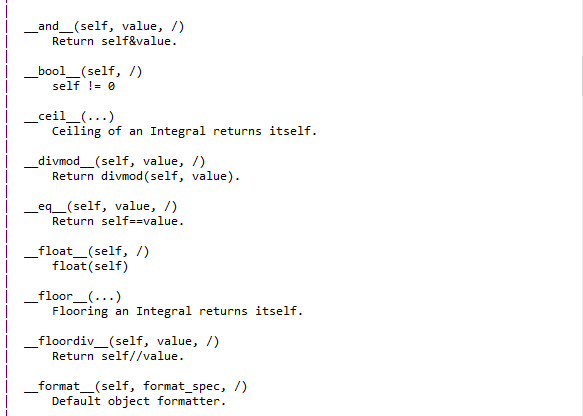
\includegraphics[width=4cm]{figures/kelompok3/1/2.png}
        \centering
        \caption{Hasil Dari Help bagian 2}
    \end{figure}
    \begin{figure}[H]
        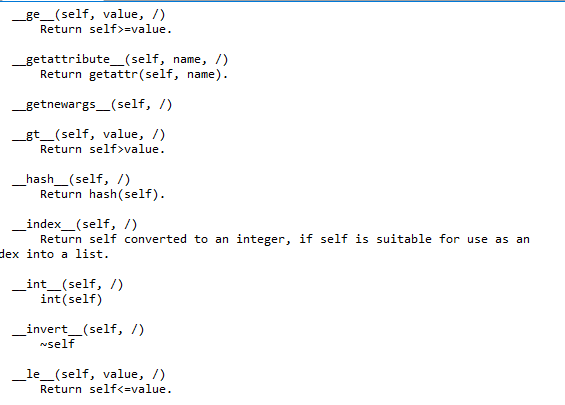
\includegraphics[width=4cm]{figures/kelompok3/1/3.png}
        \centering
        \caption{Hasil Dari Help bagian 3}
    \end{figure}
    \begin{figure}[H]
        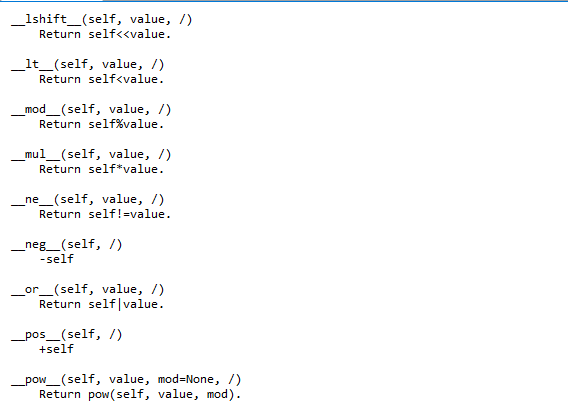
\includegraphics[width=4cm]{figures/kelompok3/1/4.png}
        \centering
        \caption{Hasil Dari Help bagian 4}
    \end{figure}
    \begin{figure}[H]
        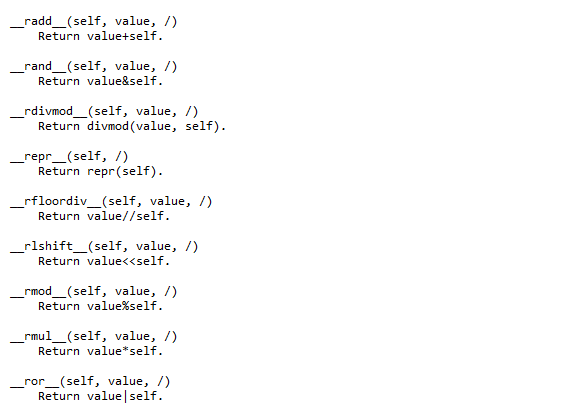
\includegraphics[width=4cm]{figures/kelompok3/1/5.png}
        \centering
        \caption{Hasil Dari Help bagian 5}
    \end{figure}
    \begin{figure}[H]
        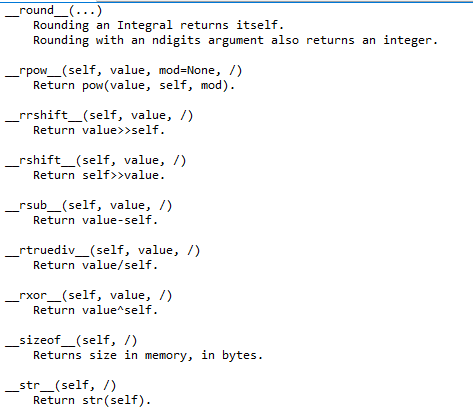
\includegraphics[width=4cm]{figures/kelompok3/1/6.png}
        \centering
        \caption{Hasil Dari Help bagian 6}
    \end{figure}
    \begin{figure}[H]
        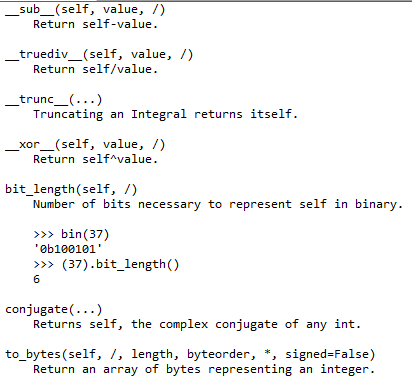
\includegraphics[width=4cm]{figures/kelompok3/1/7.png}
        \centering
        \caption{Hasil Dari Help bagian 7}
    \end{figure}
    \begin{figure}[H]
        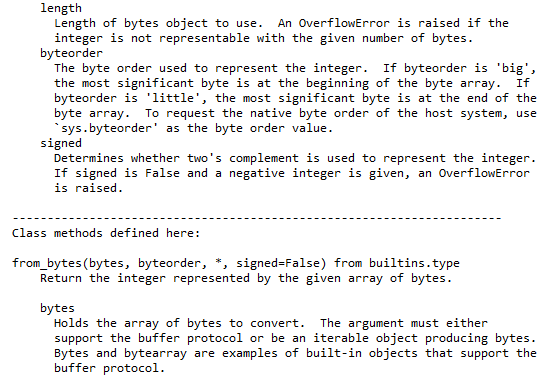
\includegraphics[width=4cm]{figures/kelompok3/1/8.png}
        \centering
        \caption{Hasil Dari Help bagian 8}
    \end{figure}
    \begin{figure}[H]
        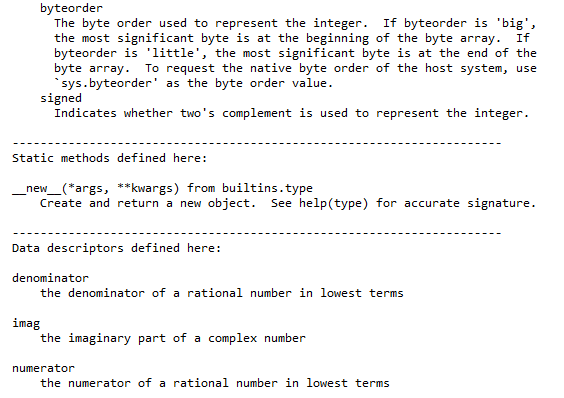
\includegraphics[width=4cm]{figures/kelompok3/1/9.png}
        \centering
        \caption{Hasil Dari Help bagian 9}
    \end{figure}
    \begin{figure}[H]
        
\includegraphics[width=4cm]{figures/kelompok3/1/10.png}
        \centering
        \caption{Hasil Dari Help bagian 10}
    \end{figure}
    \item dir(object)
    \lstinputlisting[firstline=9, lastline=10]{src/kelompok3/1/1.py}
    \begin{figure}[H]
        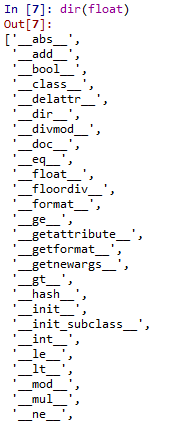
\includegraphics[width=4cm]{figures/kelompok3/1/11.png}
        \centering
        \caption{Hasil Dari Dir Bagian 1}
    \end{figure}
    \begin{figure}[H]
        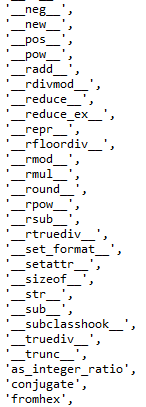
\includegraphics[width=4cm]{figures/kelompok3/1/12.png}
        \centering
        \caption{Hasil Dari Dir Bagian 2}
    \end{figure}
    \begin{figure}[H]
        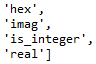
\includegraphics[width=4cm]{figures/kelompok3/1/13.png}
        \centering
        \caption{Hasil Dari Dir Bagian 3}
    \end{figure}
    \item abs document
    \lstinputlisting[firstline=11, lastline=12]{src/kelompok3/1/1.py}
    \begin{figure}[H]
        
\includegraphics[width=4cm]{figures/kelompok3/1/14.png}
        \centering
        \caption{Hasil Dari abs document}
    \end{figure}
\end{enumerate}
\section{npm - nama}
\subsection{kalo perlu}